\documentclass[journal,12pt,twocolumn]{IEEEtran}
\usepackage[none]{hyphenat}
\usepackage{graphicx}
\usepackage{listings}
\usepackage[english]{babel}
\usepackage{graphicx}
\usepackage{caption} 
\usepackage{amsmath}
\usepackage{hyperref}
\usepackage{booktabs}
\usepackage{array}
\usepackage{stix}


\title{\textbf{\\Line Assignment}}
\author{kanekal kousar}
\date{September 2022}

\providecommand{\norm}[1]{\left\lVert#1\right\rVert}
\providecommand{\abs}[1]{\left\vert#1\right\vert}
\let\vec\mathbf
\newcommand{\myvec}[1]{\ensuremath{\begin{pmatrix}#1\end{pmatrix}}}
\newcommand{\mydet}[1]{\ensuremath{\begin{vmatrix}#1\end{vmatrix}}}
\providecommand{\brak}[1]{\ensuremath{\left(#1\right)}}

\begin{document}
\maketitle


\section{Question}
\textbf{\textit{Class 11, Exercise 10.1, Q(9):} Without using distance formula, show that points (– 2, – 1), (4, 0), (3, 3) and (–3, 2)are the vertices of a parallelogram.}

\section{Solution}
\raggedright 

\begin{figure}[h!]
\centering
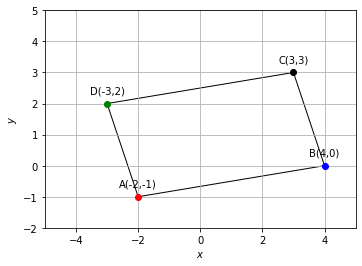
\includegraphics[scale=0.5]{fig/paralellogram.png}  
\caption{paralellogram ABCD}
\end{figure}

\vspace{0.25cm}
We can prove that the points are the vertices of a parallelogram if the direction vectors of opposite lines are equal

Consider  figure I,where


$\vec{A}=\begin{pmatrix}-2 \\ -1 \\ \end{pmatrix}\hspace{0.3cm} \vec{B}=\begin{pmatrix} 4\\ 0 \\\end{pmatrix}$

$\vec{C}=\begin{pmatrix}3 \\ 3 \\ \end{pmatrix}$ \hspace{0.3cm} $\vec{D}=\begin{pmatrix}-3 \\ 2 \\ \end{pmatrix}$ 
\vspace{0.2cm}


let the direction vector be
\begin{align}
 \vec{P} =\vec{B}-\vec{A}=\begin{pmatrix}6 \\ 1 \\ \end{pmatrix}
\end{align}
  \hspace{0.3cm}
\begin{align}  
   \vec{Q}=\vec{C}-\vec{D}=\begin{pmatrix}6 \\ 1 \\ \end{pmatrix}
\end{align}
\begin{align}
\vec{R}=\vec{A}-\vec{C}=\begin{pmatrix}1 \\ -3 \\ \end{pmatrix}
 \hspace{0.3cm}
\end{align} 
\begin{align}
 \vec{S}=\vec{A}-\vec{D}=\begin{pmatrix}1 \\ -3 \\ \end{pmatrix}
\end{align}
\unboldmath

from eq(1) and (2) $\vec{P}=\vec{Q}$

and form eq(3) and (4) $\vec{R}=\vec{S}$


since the direction vectors of opposite lines are same the points (– 2, – 1), (4, 0), (3, 3) and (–3, 2) forms the vertices of a parallelogram

\section*{Construction}
\centering
\vspace{0.2cm}
{
\setlength\extrarowheight{2pt}
\begin{tabular}{|c|c|c|}
	\hline
	\textbf{Symbol}&\textbf{Value}&\textbf{Description}\\
	\hline
	A & $\begin{pmatrix}-2 \\ -1 \\ \end{pmatrix}$ & Vertex A\\
	\hline
	B & $\begin{pmatrix}4 \\ 0 \\ \end{pmatrix}$ & Vertex B\\
	\hline
	C &$\begin{pmatrix}3 \\ 3 \\ \end{pmatrix}$ & Vertex C\\
	\hline
	D & $\begin{pmatrix}-3 \\ 2 \\ \end{pmatrix}$ & Vertex D\\
	\hline
	P &$\begin{pmatrix}1 \\ 6 \\ \end{pmatrix}$&vector AB\\
	\hline
	Q&$\begin{pmatrix}1 \\ 6 \\ \end{pmatrix}$&vector DC\\
	\hline
	R&$\begin{pmatrix}1 \\ -3 \\ \end{pmatrix}$&vector BC\\
	\hline
	S&$\begin{pmatrix}1 \\ -3 \\ \end{pmatrix}$&vector AD\\
	\hline
\end{tabular}
}

\vspace{0.6cm}
Get the python code of the figures from
\begin{table}[h]
\large
\centering
\framebox{
\url{https://github.com/kkousar/KOUSAR_FWC/blob/main/line_assignment/code/line.py}}
\bibliographystyle{ieeetr}

\end{table}



\end{document}
